\subsection{\textbf{Analisando Gráficos:}}

Os dados mostram padrões interessantes. Nos anos de Halving, vemos sempre uma valorização no logo após o começo dos anos, um acontecimento conhecido como "pre-halving uptrend", ou em português, "Tendência de alta pré-Halving". O que mostra uma valorização pouco meses antes do previsto do Evento Halving realmente acontecer. 

Vemos na \cref{fig:Candle Graph} muito bem as tendências de valorização. É possível visualizar melhor devido as proporções  maiores nos anos de 2020 e de 2024. Contudo podemos aplicar a mais eventos.

\begin{figure}[h]
    \centering
    \shadowbox{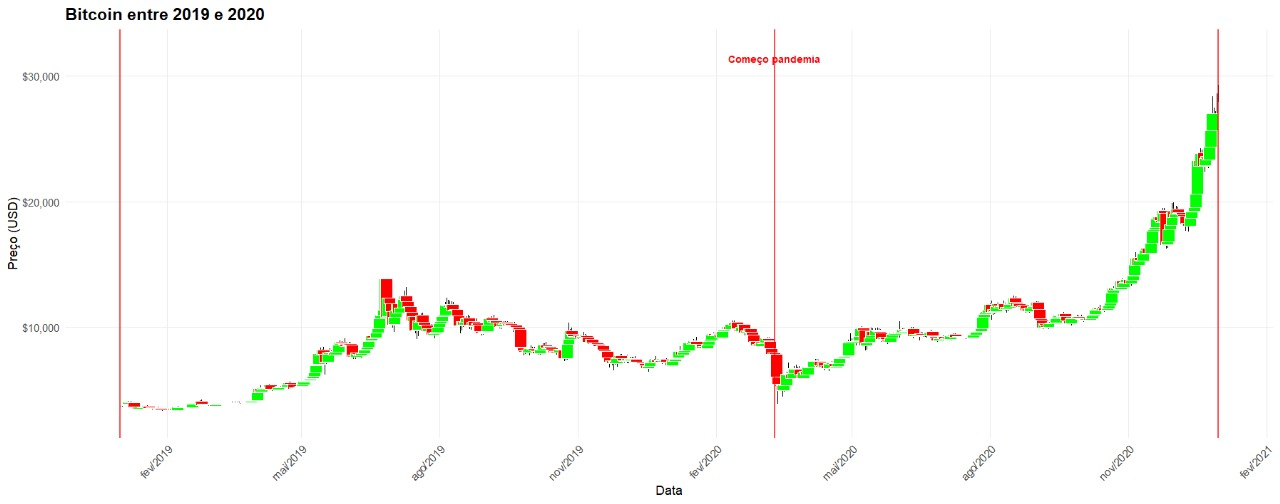
\includegraphics[width=0.8\linewidth]{Imagens/Grafico_pre_pandemia.jpg}}
    \caption{Gráfico Pré Pandemia}
    \label{fig:pre pandemia}
\end{figure}

Vindo de antes da Pandemia do COVID-19, em meados de janeiro de 2019, que a popularidade do Bitcoin estava baixa. Começou a crescer perto de junho, devido também a outros fatores também, mas principalmente por conta da euforia da pré-Halving. O seu valor de mercado permaneceu com valores instáveis, valorizando e desvalorizando com irregularidade. 

É perceptível uma queda brusca em abril de 2020 devido à pandemia de COVID-19, mas isso não perdurou por muito tempo, voltando ao seu valor habitual poucos meses depois. Entretanto, como podemos ver na \cref{fig:pandemia}, o seu maior crescimento foi quando se aproximava de 2021, que foi o começo da onda de percepção do Bitcoin como um ativo seguro contra a inflação.

\newpage

\subsection{\textbf{Análise dos Testes de Correlação}}

% Gráficos de correlação
\begin{figure}[ht]
  \centering
  \begin{minipage}{0.48\linewidth}
    \centering
    \shadowbox{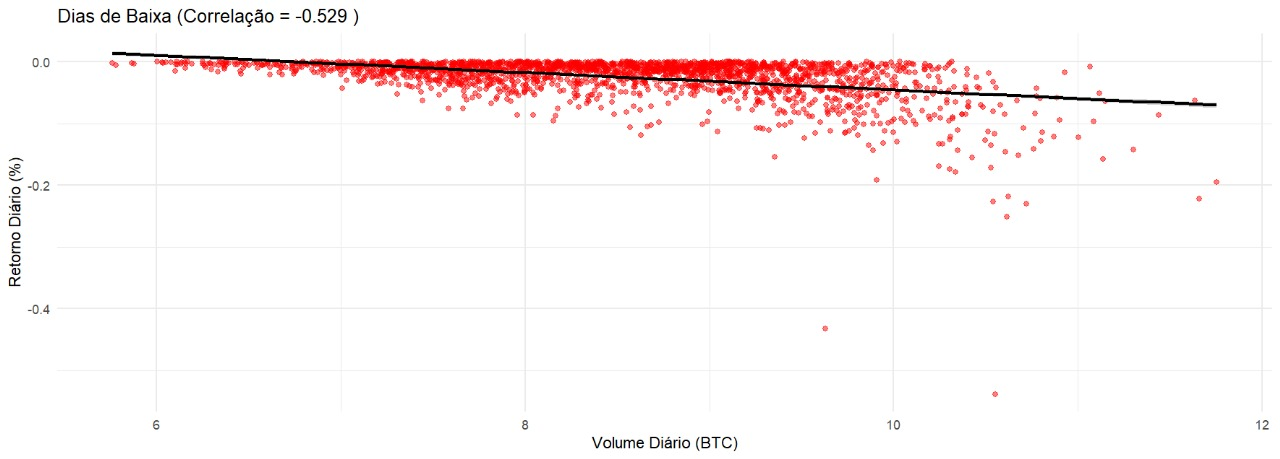
\includegraphics[width=\linewidth]{Imagens/Correlacao Negativa.jpg}}
    \caption{Gráfico de Correlação Negativa}
    \label{fig:correlacao-negativa}
  \end{minipage}\hfill
  \begin{minipage}{0.48\linewidth}
    \centering
    \shadowbox{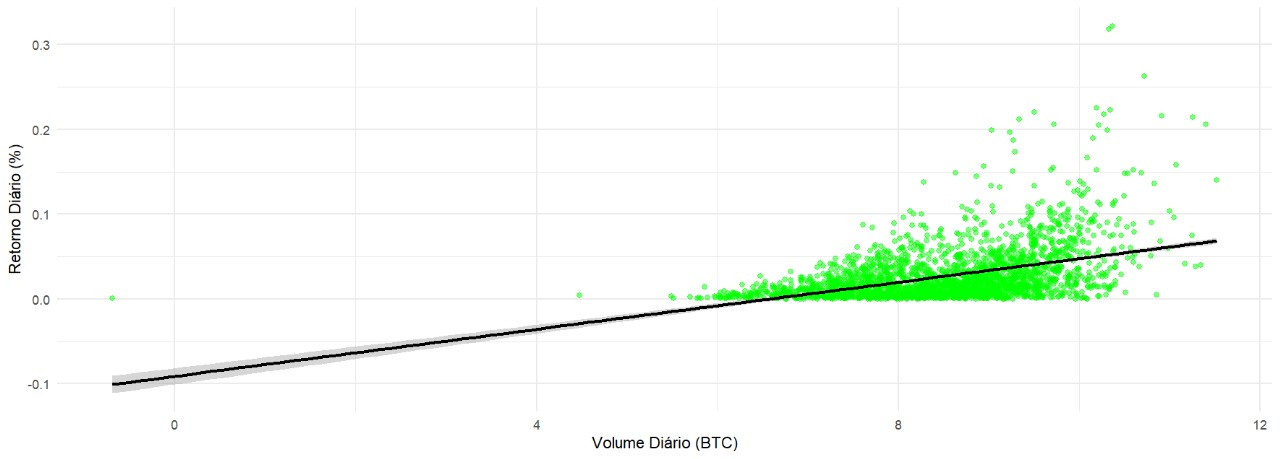
\includegraphics[width=\linewidth]{Imagens/Correlacao Positiva.jpg}}
    \caption{Gráfico de Correlação Positiva}
    \label{fig:correlacao-positiva}
  \end{minipage}
\end{figure}

Definiremos as hipóteses para 


\subsubsection{Definição das Hipóteses}
\begin{itemize}
  \item \textbf{Hipótese nula (H$_0$):} $\rho = 0$ — Sem correlação linear entre retorno diário e volume.
  \item \textbf{Hipótese alternativa (H$_A$):} $\rho \neq 0$ — Há uma correlação linear entre retorno diário e volume.
\end{itemize}

\subsubsection{Dias de Alta}
\begin{itemize}
  \item \textbf{Coeficiente de correlação (r):} $0,493$  
    Indica correlação moderadamente positiva entre retorno e volume em dias de valorização.
  \item \textbf{Estatística $t$:} $t = 27{,}902$ com 2\,421 graus de liberdade.  
    Valor elevado reforça a evidência \textbf{contra H$_0$}.
  \item \textbf{p-valor:} $p < 2{,}2\times10^{-16}$  
    Praticamente zero — altamente significativo. Rejeitamos H$_0$.
  \item \textbf{Intervalo de confiança 95\%:} $[0,463,\;0,523]$  
    Com 95\% de confiança, a correlação verdadeira está neste intervalo.
\end{itemize}

\paragraph{Interpretação.}
Em dias de alta, volume e retorno crescem juntos, sugerindo que movimentos de valorização atraem maior interesse comprador.

\subsubsection{Dias de Baixa}
\begin{itemize}
  \item \textbf{Coeficiente de correlação (r):} $-0,529$  
    Indica correlação moderadamente negativa entre retorno e volume em dias de desvalorização.
  \item \textbf{Estatística t:} $t = -28{,}574$ com 2\,102 graus de liberdade.  
    Magnitude elevada (sinal negativo indica direção inversa) reforça evidência contra H$_0$.
  \item \textbf{p-valor:} $p < 2{,}2\times10^{-16}$  
    Altamente significativo — rejeitamos H$_0$.
  \item \textbf{Intervalo de confiança 95\%:} $[-0,559,\;-0,497]$  
    Com 95\% de confiança, a correlação populacional verdadeira é negativa e está neste intervalo.
\end{itemize}

\paragraph{Interpretação.}
Em dias de baixa, o aumento de volume acompanha quedas de preço, caracterizando vendas em pânico ou liquidações forçadas.

\subsubsection{Considerações Finais}
Os resultados mostram uma assimetria de mercado:
\begin{itemize}
  \item Em \emph{alta}, maior volume ocorre junto a retornos positivos (pressão compradora).
  \item Em \emph{baixa}, maior volume ocorre junto a retornos negativos (vendas aceleradas).
\end{itemize}
Esse padrão assimétrico é relevante para modelagem de risco e elaboração de estratégias de portfólio.
